\begin{frame}{Página web Rectángulos 01/04}
\justifying
Muestra cuatro rectángulos con el fin de ilustrar varios conceptos de dibujo. Al examinar la página web, describiremos cómo dibujar un rectángulo y especificaremos su posición, altura, ancho, color y ancho del borde.

\begin{figure}[H]
\centering
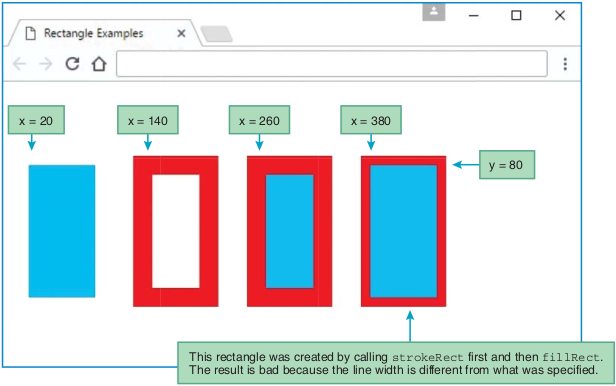
\includegraphics[scale=0.3]{Section_Files/images/Sec01/03.png}
\end{figure}

{\tiny Web Programming with html5, css, and javascript de John Dean (2019), pág. 573}
\end{frame}

\begin{frame}{Página web Rectángulos 02/04}
\justifying
\begin{figure}[H]
\centering
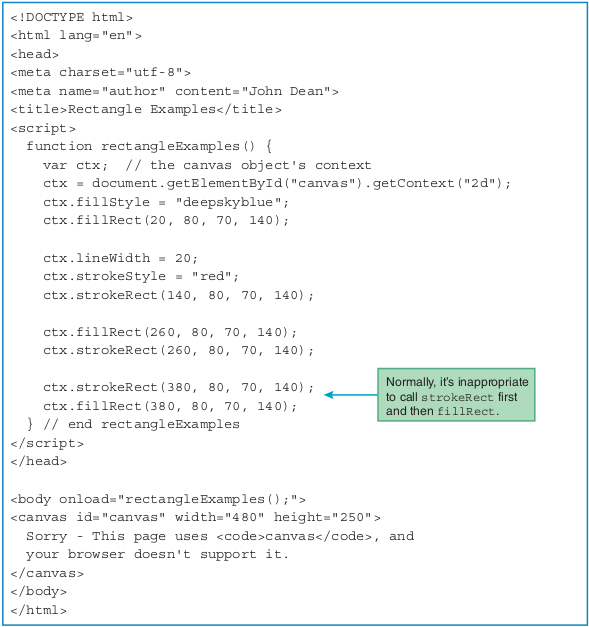
\includegraphics[scale=0.3]{Section_Files/images/Sec01/04.png}
\end{figure}

{\tiny Web Programming with html5, css, and javascript de John Dean (2019), pág. 573}
\end{frame}

\begin{frame}{Página web Rectángulos 03/04}
\justifying
Regrese a la ventana del navegador de la página web Rectángulos y observe que los rectángulos primero, tercero y cuarto tienen interiores llenos de azul. Para dibujar un rectángulo relleno, utiliza el objeto de contexto para llamar al método fillRect. Aquí está la sintaxis:

\begin{figure}[H]
\centering
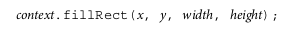
\includegraphics[scale=0.4]{Section_Files/images/Sec01/05.png}
\end{figure}

{\tiny Web Programming with html5, css, and javascript de John Dean (2019), pág. 574}
\end{frame}

\begin{frame}{Página web Rectángulos 04/04}
\justifying
Los argumentos x e y son enteros que especifican la posición de coordenadas x, y de la esquina superior izquierda del rectángulo que se va a dibujar. Si x es igual a 0 e y es igual a 0, entonces la esquina superior izquierda del rectángulo coincidirá con la esquina superior izquierda del área del lienzo. Los argumentos de ancho y alto son enteros que especifican el ancho y el alto del rectángulo. Para los valores de posición xey, y los valores de dimensión de ancho y alto, JavaScript asume unidades de píxeles y no especifica unidades explícitamente.

{\tiny Web Programming with html5, css, and javascript de John Dean (2019), pág. 574}
\end{frame}

\begin{frame}{Fill Color 01/05}
\justifying
Aquí está el código que dibuja el primer rectángulo en la página web Rectángulos:

\begin{figure}[H]
\centering
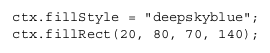
\includegraphics[scale=0.4]{Section_Files/images/Sec02/10.png}
\end{figure}


{\tiny Web Programming with html5, css, and javascript de John Dean (2019), pág. 574}
\end{frame}

\begin{frame}{Fill Color 02/05}
\justifying
La variable ctx contiene el objeto de contexto para el área de dibujo del lienzo de la página web. Observe cómo asignamos "deepskyblue" a la propiedad fillStyle del objeto de contexto. Cuando asigna un valor a la propiedad fillStyle del objeto de contexto, significa que las siguientes llamadas al método de dibujo de forma utilizarán el color especificado al rellenar la forma dibujada. Entonces, en el código anterior, cuando el objeto de contexto llama al método fillRect, el motor de JavaScript dibuja un rectángulo con un color de relleno de azul cielo profundo. Vea la ventana del navegador y observe el azul para los colores de relleno de los rectángulos.
Mientras lo hace, tenga en cuenta la posición y el tamaño del primer rectángulo y verifique que se desprenden de los argumentos 20, 80, 70 y 140 de la llamada al método fillRect. Recuerde que los dos primeros argumentos especifican la posición del rectángulo en relación con las áreas de dibujo del lienzo. Con valores de 20 y 80, la esquina superior izquierda del primer rectángulo se coloca 20 píxeles a la derecha del borde izquierdo del área del lienzo y 80 píxeles hacia abajo desde el borde superior del área del lienzo. Los siguientes dos argumentos especifican las dimensiones del rectángulo. Con valores de 70 y 140, el ancho del primer rectángulo es de 70 píxeles y su altura es de 140 píxeles.


{\tiny Web Programming with html5, css, and javascript de John Dean (2019), pág. 574}
\end{frame}

\begin{frame}{Fill Color 03/05}
\justifying
El color de dibujo predeterminado es el negro. Asignar un valor a la propiedad fillStyle cambia el color de relleno, y el motor de JavaScript usa ese nuevo color para todas las formas dibujadas en el futuro hasta que el navegador ejecute una nueva asignación fillStyle. La propiedad fillStyle afecta no solo a formas estándar como rectángulos y círculos, sino también a caracteres de texto.

{\tiny Web Programming with html5, css, and javascript de John Dean (2019), pág. 574}
\end{frame}

\begin{frame}{Fill Color 04/05}
\justifying
Al asignar colores para formas de lienzo, puede usar cualquiera de los formatos de valor de color presentados anteriormente en el capítulo CSS. Aquí están los formatos válidos:

\begin{itemize}
\item nombre de color.
\item Valor RGB: especifica cantidades de rojo, verde y azul.
\item Valor RGBA: especifica RGB, más la cantidad de opacidad.
\item Valor HSL: especifica cantidades de matiz, saturación y luminosidad.
\item HSLA: especifica HSL, más la cantidad de opacidad.
\end{itemize}

{\tiny Web Programming with html5, css, and javascript de John Dean (2019), pág. 574}
\end{frame}

\begin{frame}{Fill Color 05/05}
\justifying
Para los formatos RGB, los valores rojo, verde y azul deben ser (1) tres enteros entre 0 y 255 o (2) tres porcentajes entre 0\% y 100\%. Para los formatos HSL, los valores de matiz, saturación y luminosidad deben ser un número entero entre 0 y 360 (para grados en la rueda de color de matiz), un porcentaje entre 0\% y 100\% y otro porcentaje entre 0\% y 100\%. El rango válido para la opacidad es un número entre 0.0 (completamente transparente) y 1.0 (completamente opaco).


{\tiny Web Programming with html5, css, and javascript de John Dean (2019), pág. 574}
\end{frame}

\begin{frame}{Bordes de rectángulo 01}
\justifying
Mire nuevamente la ventana del navegador de la página web Rectángulos, y esta vez observe los bordes rojos alrededor del segundo, tercer y cuarto rectángulos. Para dibujar un borde rectangular, use el método strokeRect del objeto de contexto. Aquí está su sintaxis:

\begin{figure}[H]
\centering
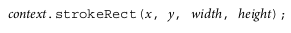
\includegraphics[scale=0.4]{Section_Files/images/Sec02/11.png}
\end{figure}

{\tiny Web Programming with html5, css, and javascript de John Dean (2019), pág. 575}
\end{frame}

\begin{frame}{Bordes de rectángulo 02}
\justifying
Los argumentos x, y, ancho y alto funcionan igual que con el método fillRect.
Aquí está la llamada al método strokeRect para dibujar el segundo rectángulo de la página web Rectangle:

\begin{figure}[H]
\centering
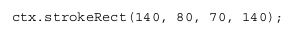
\includegraphics[scale=0.4]{Section_Files/images/Sec02/12.png}
\end{figure}


{\tiny Web Programming with html5, css, and javascript de John Dean (2019), pág. 575}
\end{frame}

\begin{frame}{Bordes de rectángulo 03}
\justifying
Si vuelve a la ventana del navegador, puede ver que la esquina superior izquierda del segundo rectángulo está justo arriba y a la izquierda del punto x = 140, y = 80 especificado por la llamada al método strokeRect.\\
¿Por qué no se coloca la esquina del rectángulo en el punto x = 140, y = 80 con precisión? Si el ancho del borde era de 1 píxel, entonces la esquina superior izquierda del rectángulo estaría en x = 140, y = 80. Pero con un borde grueso, la mitad va fuera del borde del rectángulo especificado y la otra mitad va en el interior.

Aquí está el código que aparece justo encima de la llamada al método strokeRect del segundo rectángulo:

\begin{figure}[H]
\centering
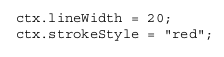
\includegraphics[scale=0.4]{Section_Files/images/Sec02/13.png}
\end{figure}

{\tiny Web Programming with html5, css, and javascript de John Dean (2019), pág. 575}
\end{frame}